\section{Input/output}
      
      In our model the "world", or landscape, is represented by a rectangular grid of alterable dimensions $N \times N$, where $N$ can be as large as 2000.
      We designed the code in a way such that it can read in an ASCII file that contains a set of numbers, those being either 0 or 1 and representing water and land, respectively, parses them and stores in a two-dimensional array. This means that the code can be used to model landscapes of different sizes with various distributions of land and water. After the input file is read into an array the number of nearest neighbours each cell has is calculated and stored in a new two dimensional array. Water cells are held as -1 so that they can be distinguished from land cells with no neighbours. This array of neighbours is all that is required by the rest of the program.
      \newline{}
      The boundary conditions are assigned to the model by setting the values for density of both, pumas and hares, to 0 at the edges of the grid.  Initially, pumas and hares are randomly distributed across the land cells. 
      All these tasks are implemented in methods within the MapReader class.
      \newline{}
      The initial values for parameters that appear in the PDE's governing the evolution of the system with time can be set up by the user, who will be able to interact with the program by means of a GUI. Specifically, it is allowed for the user to initialise the values for the birth, death and diffusion rates of both types of animals as well as the time step ($dt$), which controls how often the system is updated with new data.  The user can also control the frequency of creating the output files, by choosing a value for the parameter $T$ in the GUI window. The output gets created every $T$ time steps. We have also included an optional "range" feature which allows the user to set a range of initial values for all the differential coefficients and an increment. In this case the code will run several times creating separate outputs for every simulation. In the next section we talk about the GUI in more detail. 
      \newline{}
      Alternatively, the user can execute the code directly from within the terminal by specifying two arguments. The first argument required is the name of the file containing initial values for all the parameters, and the second is the name of the input ASCII file that will be used to create the grid. 
      \newline{}
      \newline{}
      
      The methods responsible for creating the output are included in the Output class. Depending on the user's preference, the code will create one output directory (for single initial values) or a number of such directories (for the range of initial values), i.e. one for each run. In both cases the user will be able to view the distribution of both populations across the landscape every $T$ time steps. The form of the output is a number of ppm files which can be viewed as images, or "maps", similar to these showed in the figure below.
     
      
      \begin{figure}[H]
      \begin{center}
  \subfloat[$t=360$]{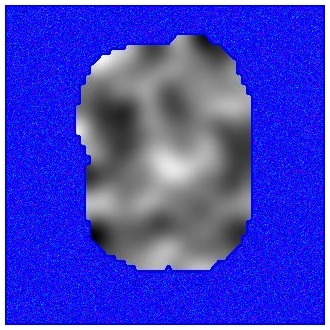
\includegraphics[width=55mm]{figs/Puma900.jpg}}
  \subfloat[$t=416$]{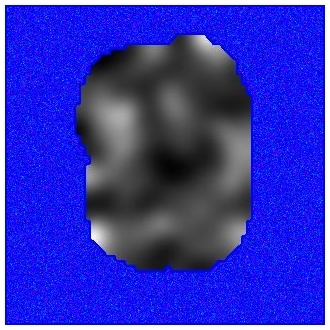
\includegraphics[width=55mm]{figs/Puma1040.jpg}}
      \caption{This figure shows examples of the output files created during a simulation using a $500 \times 500$ grid and default initial conditions. Various shades of grey represent the density of pumas after 900 (a) and 1040 (b) time steps, with time step size set to 0.4.}
      \end{center}
      \end{figure}
      
     
      The number of the ppm files created depends on the initial parameters specified by the user, $dt$ and $T$. To maximise the level of output clarity we decided to make separate landscape "maps" for each type of animal, here pumas and hares. In each "map" the pixels corresponding to water cells are shown in blue, while the land cells are white. The variation in density of pumas/hares across the land cells is represented by different shades of grey, with black colour corresponding to the maximum value. 
      \newline{}
      For each type of animal, every $T$ time steps, the code also calculates the mean population density and writes it along with the corresponding time into a file. 
